\documentclass[../main.tex]{subfiles}

\begin{document}
	\section{Structure des polymères à l'état solide}
	Comme les petites molécules, certains polymères sont cristallins. Cependant il ne sont jamais à 100\% cristallins. Les polymères qui peuvent se cristalliser sont dénommés comme \textbf{semi-cristallin}. La micro-structure des polymères semi-cristallins se compose de cristaux polymères entourés par une matrice polymères amorphe (fig. \ref{amorphe}). 
	\begin{figure}[h]
		\begin{center}
			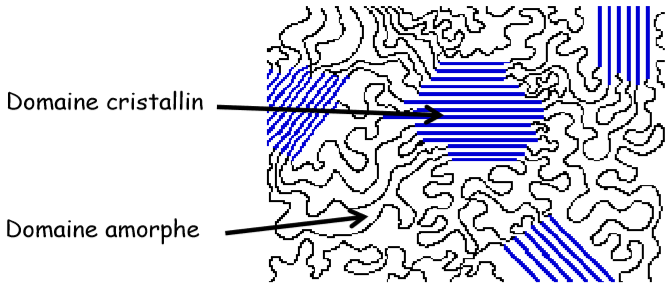
\includegraphics[scale=1]{Amorphe.png}
			\caption{\label{amorphe}Représentation des micro-structures d'un polymère semi-cristallins}
		\end{center}
	\end{figure}
	Les polymères n'ayant pas la possibilité de former des domaines cristallins se composent uniquement d'une phase amorphe et sont ainsi dénommés \textbf{polymères amorphes}.
	
	La dégradabilité ne dépend pas uniquement de la micro-structure du polymère, sa masse moléculaire ou encore sa polarité, mais ces paramètres sont souvent corrélés.
	\\
	La phase cristalline est caractérisée par un \textbf{point de fusion}, c'est à dire la température à laquelle le domaine cristallin fond. 
	
	\subsection{Phase des polymères à l'état solide}
	
	\begin{figure}[h]
		\begin{center}
			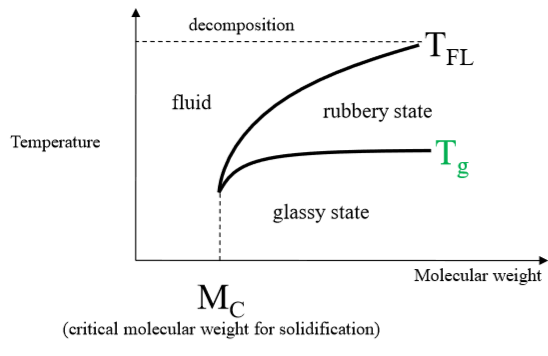
\includegraphics[scale=1]{PolyPhase.png}
			\caption{\label{polyphase}Etat d'un polymère en fonction de sa masse molécule et de sa température}
		\end{center}
	\end{figure}

	Un polymère amorphe peut généralement adopter 3 états distincts. Le nombre de phases atteignable pour un polymère ainsi que les températures de transition entre ces phases dépend de sa masse moléculaire (fig. \ref{polyphase}). 
	
	\section{Polymères amorphes vitreux}
	
	\subsection{La conformation statistique}
	\begin{figure}[h]
		\begin{center}
			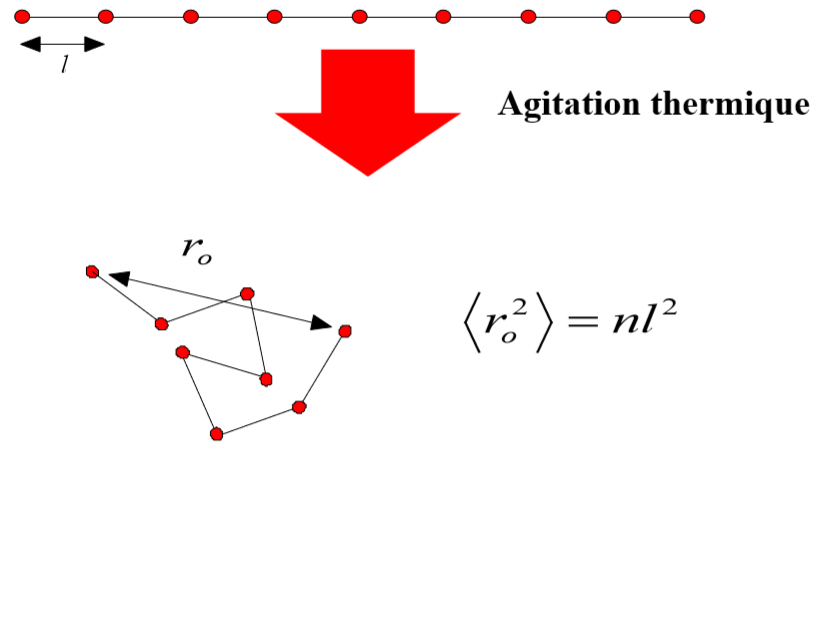
\includegraphics[width=18cm]{AmorpheVitreux.png}
			\caption{\label{amorphevitreux}Cas d'une chaîne à \textit{articulation libres} isolée}
		\end{center}
	\end{figure}

	Une chaîne isolée va adopter une conformation en \textit{pelote} statistique (qui change toutes les $10^-12$ secondes). Tel que montré sur la figure \ref{amorphevitreux}, on trouve $n$ le nombre de liaisons. $<r_0^2>$ est proportionnel à $M$. La taille d'une chaîne est proportionnelle à sa masse molaire. Pour les chaînes réelles, il faut respecter les angles de valence, l'encombrement stérique etc, donc en pratique on trouve $<r_0^2> > nl^2$, avec $l$ la longueur moyenne des liaisons caténaires. Pour généraliser ceci, on rajoute une constante qui permet de définir sur le polymère est souple ou rigide. 
	\begin{equation}
		<r_o^2> = C_\infty nl^2
	\end{equation}
	Pour $C_\infty = 1$, peu d'encombrement stérique, donc polymère souple. A l'inverse, pour $C_\infty >> 1$, on trouve des chaînes hautement conjuguées, donc on aura un polymère rigide. 
	
	\subsection{Conformations à l'état fondu}
	A l'état fondu, si la mobilité est suffisante, les chaînes devraient adopter les conformations en \textit{pelote} d'une chaîne idéale isolée ($<r_0^2> = C_\infty nl^2$). 
	
	\subsection{La température de transition vitreuse}
	La température de transition vitreuse $T_g$ est nommée ainsi d'après le ramollissement du verre. La température de transition vitreuse est définie comme la température à partire de laquelle les propriétés mécaniques d'un matériau polymère changent radicalement à cause du mouvement interne des chaînes polymères qui composent ce matériau. D'un point de vue moléculaire, cette transition implique le début de mouvements coordonnés de longue distance. C'est le début de la \textbf{reptation}.
	On atteint rarement l'état vitreux pour de petites molécules car la cristallisation est trop rapide. Dans les polymères, la cristallisation est lente/partielle, voire impossible dans les polymères comme le aPP, aPS, aPMMA!
	
	\subsection{Caractéristiques de la phase amorphe}
	\subsubsection{Phase vitreuse}
	Dans cette phase, le polymère se comporte comme un solide dur et cassant. Les chaînes sont rigides et il n'y a pas de rotation moléculaire, seulement des vibrations.
	\subsubsection{Phase caoutchouc}
	Dans cet état, le polymère se comporte comme un solide mou et facilement déformable. Les rotations moléculaires sont désormais possible.
	\subsubsection{Phase fluide}
	Dans cette phase, le polymère agit comme un liquide. Si la masse moléculaire du polymère est trop basse, il ne peut pas adopter les phases solides décrites ci-dessus. La transition de la phase caoutchouc à fluide est progressive et dépend de la distribution de la masse moléculaire du polymère. 
	\subsection{Facteurs qui influencent la transition vitreuse}
	\begin{itemize}
		\item \textbf{Masse molaire}, mais seulement lorsque $M$ est relativement faible. Le monomère d'un polymère vitreux peut être liquide (colles cynoacrylate, résines époxydes etc...)
		\item \textbf{Rigidité des chaînes}, les liaisons caténaires linéaires, les groupes rigides dans la chaine principale (noyaux benzéniques), groupes encombrants, interactions spécifiques intrachaîne. Plus $C_\infty$ est élevé, plus la $T_g$ augmente.
		\item \textbf{Interactions spécifiques} interchaîne, des ponts hydrogènes dans les polyamides. (plus elles sont fortes, plus la $T_g$ augmente)
		\item \textbf{Plastifiants} qui baissent la $T_g$. Il existe deux types, les internes (groupe latéraux souples) et les externes (adjuvants, souvent avec le PVC)
	\end{itemize}
	On trouve différents polymères amorphes vitreux. Dans tous les cas, $T_g > temp ambiante$, ces polymères ne se cristallisent pas pendant la mise en oeuvre. 
	\begin{itemize}
		\item Polystyrène atactique (aPS)
		\item Poly chlorure de vinyle atactique (aPVC)
		\item Poly méthacrylate de métyhle atactique (aPMMA)
		\item Polycarbonate (PC)
		\item Divers thermodurcis (époxides par exemple)
	\end{itemize}
	
	Les valeurs typiques de $T_g$ varient généralement entre $190K$ et $350K$
	\subsection{Application des polymères amorphes vitreux}
	Les polymères amorphes vitreux sont des solides durs, assez rigides ($2-3GPa$ typiquement) bien que beaucoup moins que les aciers ou les verres silicate. Ils sont plastique et cassant (par exemple le PS) et son transparents (car amorphes), en effet, il n'ont pas la structure pour diffuser la lumière et ils n'ont pas d'absorption. Néanmoins on peut les rendre opaques par charges minérales et/ou pigments.
	\section{Polymères semi-cristallins}
	On peut voir un exemple de polymère semi-cristallin à la figure \ref{amorphe}. Un polymère possède un degré de cristallinité, noté $X_c$. On peut représenter un diagramme schématique pour un polymère semi-cristallin (fig. \ref{diagrammecristallin}).

	\begin{figure}
		\begin{center}
			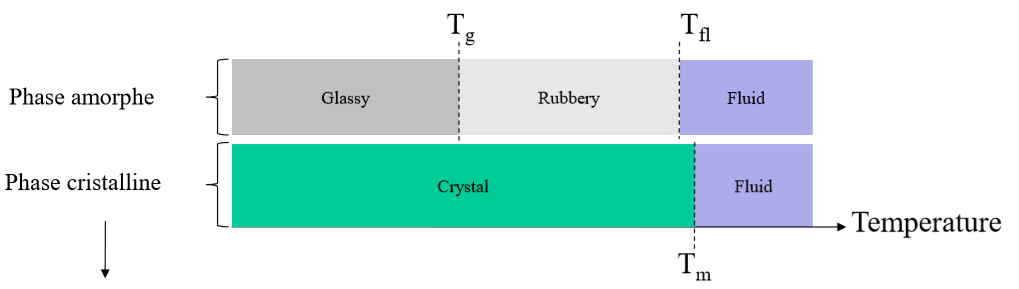
\includegraphics[width=16cm]{DiagrammeCristallin.png}
			\caption{\label{diagrammecristallin}La quantité relative de phase amorphe et de phase cristalline est appelée le degrés de cristallinité $X_c$}
		\end{center}
	\end{figure} 
	Les polymères amorphes possèdent uniquement la partie supérieure de ce diagramme de phase.
	
	\subsection{Quels polymères cristallisent?}
	Les polymères thermoplastiques qui ont des propriétés mécaniques comparables à celles des polymères amorphes vitreux cristallisent en général. Malgré que la $T_g$ des polymères (semi)cristallins est souvent inférieure à la température ambiante. Ils sont en général opaques. (PET 30\% cristllin). Une liste non exhaustive des polymères qui cristallisent:
	\begin{itemize}
		\item iPP
		\item PET
		\item PPS
		\item PTFE
		\item PE (HDPE ou LDPE)
		\item POM
		\item PA6,6
		\item PEEK
	\end{itemize}

	Pour qu'un cristal (et donc une structure périodique) se crée, il faut une configuration périodique (donc une chaîne périodique). En contre exemple, les \textbf{Colopymères statistiques}, les \textbf{polymères hautement ramifiés} et les \textbf{polymères hautement réticulés} sont difficile voire impossible à cristalliser. 
	La tacticité joue un grand rôle dans la cristallisation. Les polymères \textbf{isotactiques} et \textbf{syndiotactiques} peuvent cristalliser en adoptant une conformation régulière alors que les polymères \textbf{atactiques} ne peuvent pas cristalliser (par exemple aPS, aPP, polymères amorphes) (fig.\ref{syndiotacticite}).
	
	\begin{figure}
		\begin{center}
			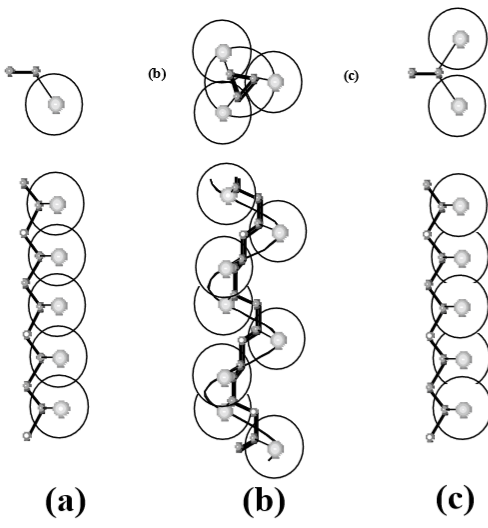
\includegraphics{Synbiotacticite.png}
			\caption{\label{syndiotacticite}De gauche à droite : Polymère isotactique, syndiotactique, isotactique. Ils peuvent facilement cristalliser.}
		\end{center}
	\end{figure}
	Attention! Le poly alcool de vinyle atactique peut cristalliser car le groupe latéral n'est pas assez grand pour perturber la conformation des chaînes. 
	\subsection{Facteur du point de fusion}
	Pour un cristal parfait, la température de fusion thermodynamique $T_fo$ est donnée par : $\Delta G = \Delta H - \Delta ST_fo = 0$. $\Delta H$ est donnée par les forces de cohésion et $\Delta S$ est donné par l'entropie de conformation. Une cohésion importante et un changement d'entropie faible conduisent à une $T_f$ élevée, cf. $T_g$.
	Le PC peut cristalliser, mais seulement très lentement et il est considéré comme un polymère amorphe car il ne cristallise pas dans les conditions de mise en oeuvre usuelles. 
	\subsection{Polymère semicristallin}
	C'est un polymère cristallisé à partir de l'état fondu ou de solutions concentrées. Le taux de cristallinité est d'environ 50\%, selon le polymère et les conditions de solidification. Le reste du polymère est à l'état amorphe (vitreux ou caoutchouc) selon la $T_g$. A la température ambiante, les régions amorphes du PE et du iPP sont caoutchoutique, donc plutôt molles. Dans le PET, le PA ou le PEEK, elles sont vitreuses. La rigidité de polymères à basse $T_g$ comme le PE et le iPP est fortement inluencée par leur taux de cristallinité, tandis que le PET, le PA ou le PEEK qui on une $T_g$ élevée sont rigides même pour un taux de cristallinité proche de 0.
	\subsection{Sphérolites}
	La microstructure d'un polymère semi-cristallin est typiquement \textit{sphérolitique}. Cela se représente comme un amas plus ou moins sphérique de matière amorphe et de matière cristalline. La $T_f$ est très sensible aux conditions de solidification. Définition de mesures de \textit{biréfringence}, Axes des chaînes de la phase cristalline orientés tangentiellement. 
	\subsection{Polymères cristallins orientés}
	Si un polymère cristallin est orienté au lieu d'être isotrope, le $\Delta S$ devient faible, et donc la cristallisation est favorisée pour le polymère orienté. On trouvera aussi peu ou pas de sphérulites, donc il sera relativement transparents (bouteilles en PET, sac en PE).
	\subsection{Application des polymères semicristallins}
	Se sont des solides plus ou moins rigides, ils sont résistants à la rupture, et aux solvants. En général opaques, surtout si de la sphérolitique est présente. 
	\subsection{Polyéthylène ultraorienté}
	L'UHMWPE est un polyéthylène à masse molaire ultra-élevée, environ $3'000'000g/mol$, il est formé à partir d'un procédé spécial dans un gel très dilué. Il possède des propriétés mécaniques comparables à celles des fibres inorganiques ($modulus = 200GPa$) tout en restant très léger. Le UHMWPE est aussi intéressant sous forme non-orienté car très résistant à l'abrasion. On le commercialise sous le nom de Spectra et Dyneema, son utilisation principale est pour les cables pour voiliers, les gilets pare-balles, les snowboards, les fils pour cerf-volant.
	
	\section{LCPs et mélanges}
	LCP ou \textit{liquid crystalline polymers} sont des polymères capables de s'orienter spontanément. Soit à l'état fondu, soit en solution. Par exemple on trouve le Kevlar ou le Vectra
	\subsection{Architectures des LCPs}
	\begin{figure}
		\begin{center}
			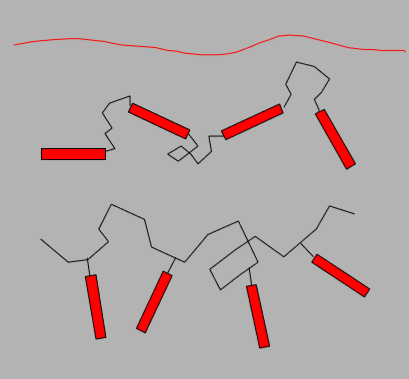
\includegraphics{Troncs.png}
			\caption{\label{LCP} Architecture en troncs d'arbre canadien sur le fleuve pour les LCPs}
		\end{center}
	
	\end{figure}
	Les LCPs sont des macromolécules globalement rigides qui contiennent des unités rigides (mésogéniques). On peut la comparer aux troncs d'arbre sur un fleuve canadien (fig. \ref{LCP}), ces molécules sous forme de bâtonnet rigide vont s'aligner les unes avec les autres. Ils possèdent de très bonne propriétés mécaniques dans le sens de l'orientation. Se sont des polymères \textit{auto renforçants}.
	\subsection{Utilisation et application}
	Ce sont des thermoplastiques auto renforçants mais leur nature leur donne aussi une faible viscosité à l'état fondu, donc permet un moulage de précision, et confère une très bonne résistance à la chaleur et aux produits chimiques. En contrepartie, ils sont très chers et ont une anisotropie parfois difficile à contrôler
	\subsubsection{Kevlar}
	Le Kevlar est seulement exploitable sous forme de fibre! Il a un module et une ténacité comparable à ceux du UHMWPE. Il possède une bonne résistance à la chaleur. Il est cher et peu résistant en flexion.
	\subsection{Miscibilité}
	La majorité des polymères ne se mélanges pas, tout comme l'huile et l'eau. Différents mélanges peuvent néanmoins améliorer les résistances à la rupture (fig. \ref{melange}).
	\begin{figure}
		\begin{center}
			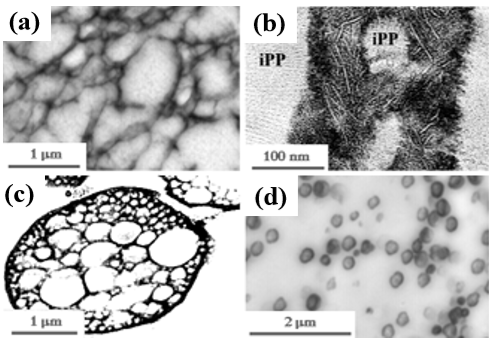
\includegraphics{Melange.png}
			\caption{\label{melange}Différents mélanges de polymère. (a) Réseau interpénétré (IPN), structure hautement réticulée à base de polyurethanne, (b) Reactor blend iPP + PP-co-PE, (c) Polymérisation en émulsion (HIPS), (d) Ajout de particules préformées et réticulées (PMMA)}
		\end{center}
	\end{figure}
	\subsection{Copolymères}
	On trouve deux grandes classes de polymères.
	Les \textbf{Copolymères aléatoires} $T_g = $moyenne des composants, $T_f$ faible ou inexistante. On trouve dans cette catégorie par exemple le polyéthylène-co-propylène et le polystyrène-co-acrylonitrile (PSAN). La deuxième catégorie se compose des \textbf{Copolymères blocs} (avec séparation de phases). Ils permettent de combiner les propriétés très différentes, par exemple élastomère et polymère vitreux dans des domaines de taille réduite. 
	\\\textbf{Question:} \\Le polystyrène et le PVC isotactiques existent, mais ce sont le PS et le PVC atactiques qui dominent le marché. Pourquoi? \\ Température $T_g$ est de environ $100 C$. Puisqu'on doit pouvoir mettre du café dedans, il est a environ 80C donc ça suffit. On a dont pas besoin d'augmenter la $T_g$ car cela coûterait plus cher.
	\subsubsection{L'ABS}
	L'ABS (acrylonitrile butadiène styrène) est un constitué d'un copolymère aléatoire d'acrylonitrile et de styrène (amorphe, vitreux, plus résistant que le PS) contenant des blocs d'un caoutchouc, le polybutadiène qui améliore sa résistance aux chocs. 
	\section{Résumé}
	\subsubsection{Amorphous glassy polymers}
	Importance de la structure chimique, rigidité, interactions spécifiques. Pour la température de transition vitreuse; ce sont des exemples de polymères amorphes. 
	\subsubsection{Semicrystalline polymers}
	Importance de la structure chimique, rigidité, interactions spécifiques, possibilité de conformations périodiques. Pour la cristabilisation et la température de fusion des polymères; ce sont des exemples de polymères qui cristallisent; ils ont la morphologie des polymères semi-cristallins (lamelle, sphérulites et autres morphologies).
	\subsubsection{LCPs}
	
	\subsubsection{Copolymères}
	Miscibilité des polymères, liaison non miscible. Des block et aléatoires copolymères. 
	 
\end{document}